\documentclass[tightenline,notitlepage,nofootinbib]{revtex4-1}

\bibliographystyle{plainnat}
%\DeclareOption{nofootinbib}{\@booleanfalse\footinbib@sw}

%\@booleanfalse\footinbib@sw

\usepackage{graphicx}
\usepackage{amsmath}
\usepackage{subcaption}
\usepackage{sidecap}
\usepackage{empheq}
\usepackage{cleveref}


\DeclareMathOperator{\erf}{Erf}
\DeclareMathOperator{\trace}{Tr}

\newcommand{\spinup}{\uparrow}
\newcommand{\spindown}{\downarrow}
\newcommand{\KSAE}{{I}}
\newcommand{\qav}[1]{\langle {#1} \rangle}
\newcommand*{\ket}[1]{\left \lvert {#1} \right \rangle}
\newcommand*{\bra}[1]{\left \langle {#1} \right \rvert}
\newcommand{\comm}[1]{{ \textbf{#1} }}



\begin{document}
  \title{An upgrade study of chargino detection with finer mass splittings.}
  \author{Janis Erdmanis \\ graphitewriter@gmail.com}
%  \email{akels14@gmail.com}
  \date{August 2016}
  \maketitle

  \section{Introduction}

  In the Standard Model (SM) Higgs mass is highly sensitive to the details of the physics at high-energy \cite{Barbieri}. Unless we accept big number cancellations, SM does not work well with naturalness principle which leads us to beyond SM (BSM) physics. This issue is resolved in supersimetry (SUSY) introducing new particles, new processes at higher energies \cite{Carlos}. With a present data from large hardron collider (LHC) \cite{PhysRevD.93.052002} we know that all superpartners should be heavy except higgsino, where lower bound is established from LEP\footnote{Large electron positron accelerator.} to be larger than $100~\rm{GeV}$, but smaller than $1 ~\rm{TeV}$ for naturalness principle to hold. Here we consider possibility to push lower bound of higgsino mass with data from high luminosity LHC at ATLAS experiment \cite{HLLHC,ATLASCOL-2008}, therefore we initialy consider higgsino mass to be $\mu=100~\rm{GeV}$ and its mass splittings $\Delta m = 5~\rm{GeV}$ (see \cref{fig:basic}).

Similarly as in previos studies \cite{PhysRevD.89.075007,ATL-PHYS-PUB-2015,PhysRevD.93.052002} here we are considering chargino, neutralino $\tilde \chi_1^{+},~\tilde \chi_1^{-}$ production which decay to neutralinos, neutrinos and soft leptons (see \cref{fig:basic}). These leptons are buried in SM background which comes from $pp\to \tau \tau + j$, $pp\to t \bar t + j$, $pp \to WW + j$ and have comparable cross-section as a signal (see \cref{tab:cross}). Also in our analysis we include process $pp \to W +j$ which although produces one lepton but because of large cross-section has a chance for incorectly detecting second lepton coming from jet (fake leptons). 
\begin{figure}[!ht]
    \centering
    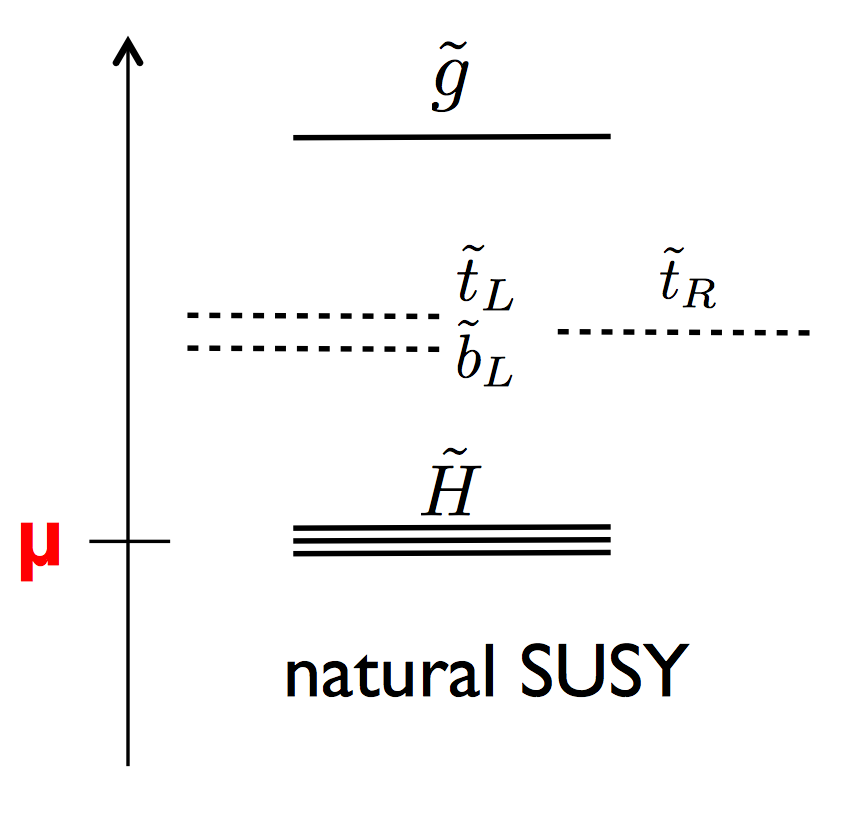
\includegraphics[width=0.25\textwidth]{splittings.png}
    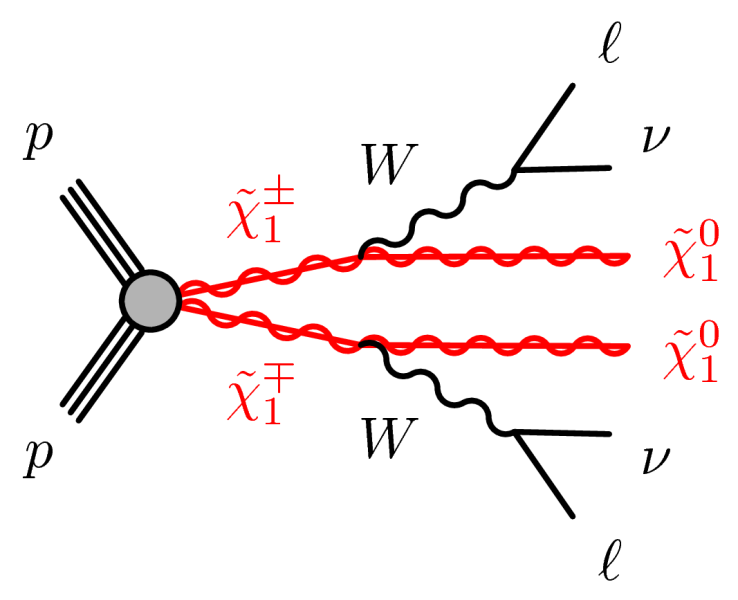
\includegraphics[width=0.25\textwidth]{C1C1.png}
    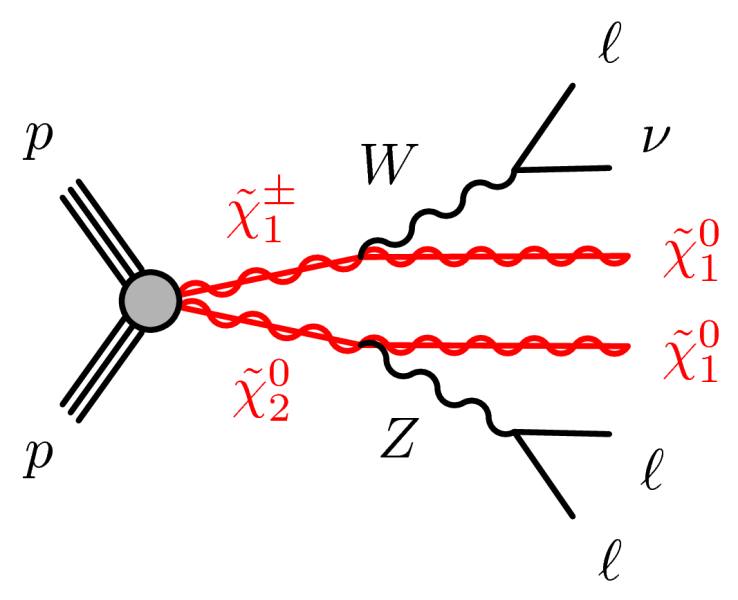
\includegraphics[width=0.25\textwidth]{C1N2.png}
    \caption{The SUSY particle mass specturm with higgsino mass $\mu$ (left), 2 soft lepton SUSY signal (middle) and 3 soft lepton SUSY signal (right).}
    \label{fig:basic}
  \end{figure}

\begin{table}[!ht]
  \centering
  \begin{tabular}{ll}
    Process & $\sigma_{eff}$ \\
    \hline
    $pp\rightarrow \tau \tau + j$ & $47.6~\rm{pb}$\\
    $pp\rightarrow t \bar t + j$ & $ 8.9~\rm{pb}$\\
    $pp \rightarrow W + j$ &  $162~\rm{pb}$ \\
    $pp \rightarrow WW +j$ & $1.34~\rm{pb}$\\
    $pp \rightarrow \tilde \chi_1^{+}\tilde \chi_1^{-} + j \rightarrow WW + j$ & $2.8~\rm{pb}$\\
    $pp \rightarrow \tilde \chi_1^{+}\tilde \chi_2^{0} + j \rightarrow WZ + j$ & $5~\rm{pb}$\\
  \end{tabular}
  \caption{Cross-sections at $14~\rm{TeV}$ for soft lepton processes}
  \label{tab:cross}
\end{table}
% MadGraph event generator for all theese processes is used from which we try to extract signal with appropriate selection.

To study and compare the signal and backgrounds, we turn to Monte Carlo. We simulate the hard processes for the signal and the major backgrounds with Madgraph 6. The parton-level events are then showered and hadronized with Pythia 8. 

\section{Simplified detector simulation}

Event reconstruction is limited by a detector imperfections, geometry, resolution and other properties. Because a real detector simulation is costly here we are going to use simplified model.

Firstly we smear energies, masses, momenta, $\eta$, $\phi$, jet labels\footnote{Because of efficiency with which we can distinguish jets from $b$-jets.} of all objects (particles and jets) with corresponding performance functions for $200$ average interactions per bunch crossing as expected in HL LHC. Then from these smeared event particles we are able to detect only ones which hit detector $|\eta|<2.8$, for leptons with transverse momenta $p_{\rm{T}} > 5~\rm{GeV} $ and for jets $p_{\rm T}>50~\rm{GeV}$. At overlap removal stage if lepton and jet are separated with less than $\Delta R = \sqrt{\Delta \phi^2 + \Delta \eta^2}<0.2$ and if transverse momenta of lepton is at least $50~ \%$ of transverse momenta of jet then we discard jet. For remaining objects if distance between jet and lepton is $\Delta R < 0.4$ we discard lepton assuming it belongs to the jet. We also assume that lepton belongs to jet if it has small energy and momenta compared to all particles around the cone. And eventually we remove low mass $<12 ~\rm{GeV}$ leptons with opposite charge, because they are affected with resonance processes not considered here.  

For checking this simplified detector simulation we plot transverse momentum of leading jet and leading lepton at different stages of algorithm (see figure \cref{fig:check}). For jets we see that smearing of variables indeed makes distribution broader (red line) where cut at $30~\rm{GeV}$ corresponds to undefined behavior of smearing function. Then some jets are removed at overlap removal stage while majority are discarded with $p_{\rm T}$ threshold (green line). Similarly for leading lepton we see considerable smearing (red line) and discarded leptons with $p_{\rm T}$ threshold and a little amount discarded at overlap removal stage (green line). 
\begin{figure}[!ht]
  \centering
  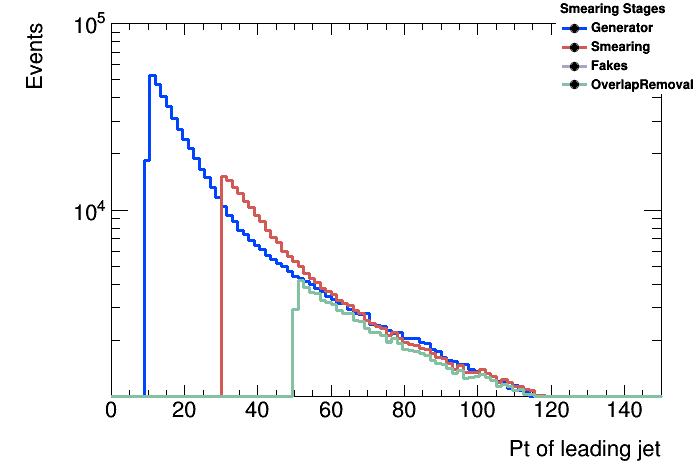
\includegraphics[width=0.45\textwidth]{h_PtJets1stStages.png}
  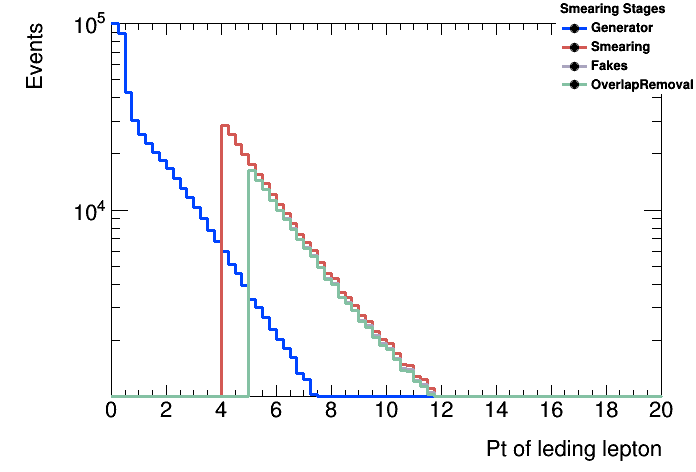
\includegraphics[width=0.45\textwidth]{h_PtEleMuo1stStages.png}
  \caption{Tests of smearing functions for signal sample C1C1 at different stages for leading jet $p_{\rm T}$ (left) and leading lepton $p_{\rm T}$ (right). Generator (blue line), smearing stage (red line) and overlap removal (green line).}
  \label{fig:check}
\end{figure}

% \begin{figure}[!ht]
%   \centering
%   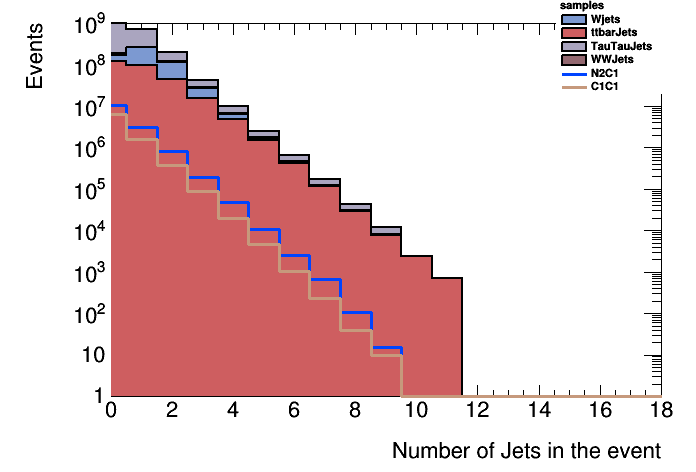
\includegraphics[width=0.25\textwidth]{h_NJet.png}
%   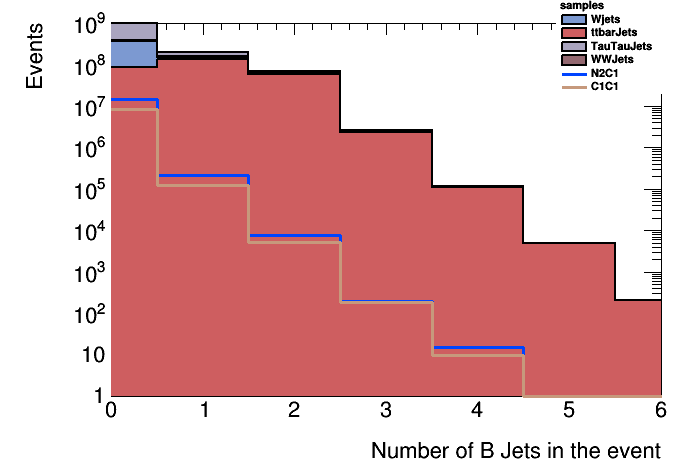
\includegraphics[width=0.25\textwidth]{h_NBJet.png}
%   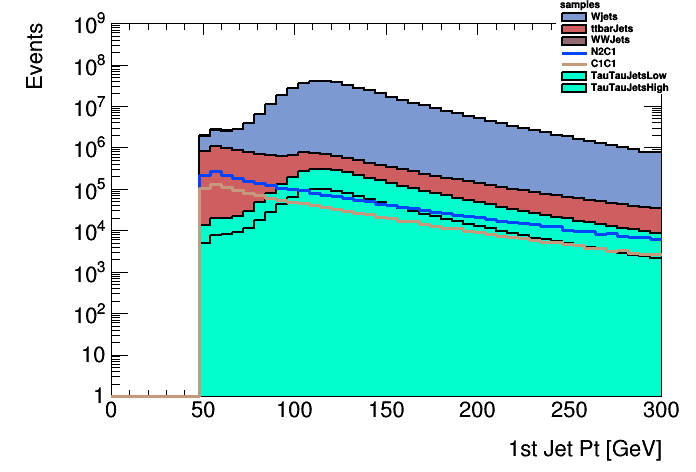
\includegraphics[width=0.25\textwidth]{h_PtJets1st.png}
%   \caption{Number of Jets, Bjets and leading jet transverse momentum.}
% \end{figure}

\section{Event selection}

Without any selection we have low signal and background relative ratio as in \cref{fig:nocuts} which also helps us to check the simulation. For example we see resonance for transverse mass at $90~\rm{GeV}$ for $pp \to W +j$ as expected. To increase signal ratio over background we are going to apply selection.
\clearpage
\begin{figure}[!ht]
  \centering
  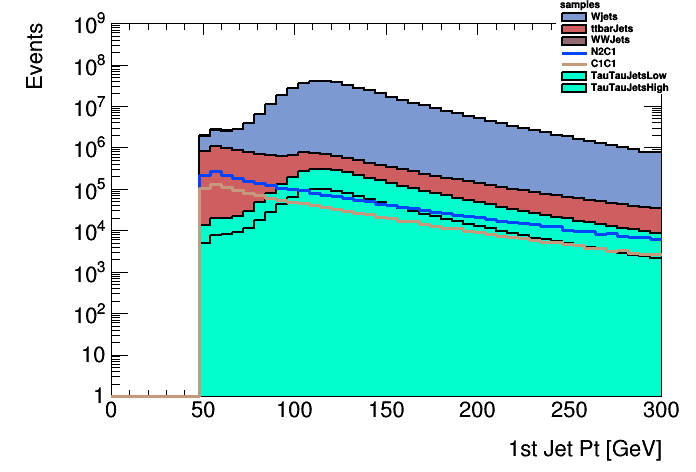
\includegraphics[width=0.3\textwidth]{h_PtJets1st.png}
  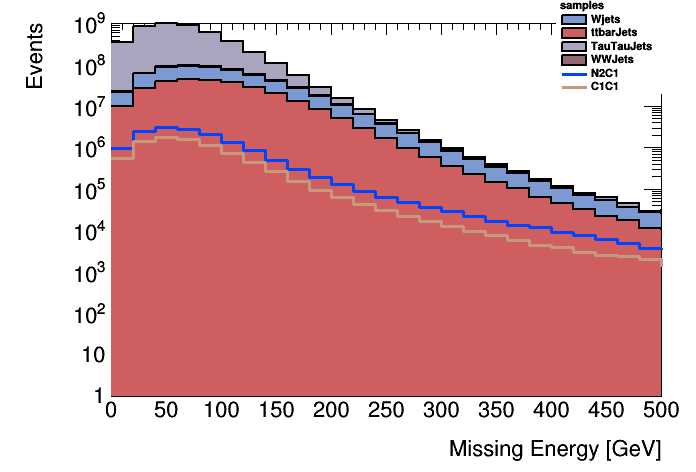
\includegraphics[width=0.3\textwidth]{h_MET.png}
  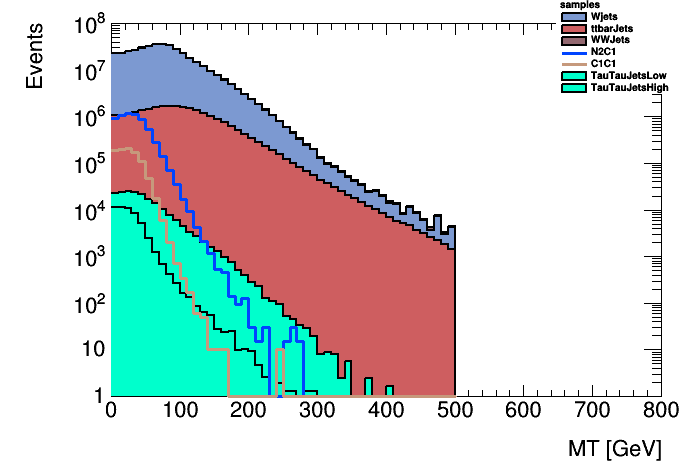
\includegraphics[width=0.3\textwidth]{h_MT.png}
  \caption{Missing energy (left), two leading lepton mass $m_{ll}$ (middle) and transverse mass (right). SUSY signals (blue and orange lines), background processes (filled green, red, blue). }
  \label{fig:nocuts}
\end{figure}

We now that in the signal leptons are soft (small transverse momenta) and neitralinos, neitralinos does not leave trace to our detector which is indirectly detected as missing energy. If we consider single jet with large transverse momentum in our process then because of transverse momentum conservation in our signal we expect large missing energy. We also know that in signal process we don't have $b$-jets so we can eliminate with it background $pp \to t \bar t + j$. Therefore selection we are considering is 
\begin{itemize}
\item $E_T^{\rm{miss}}>200~\rm{GeV}$. 
\item Single Jet with $p_{\rm T}>100~\rm{GeV}$ and no $b$-jets in event. 
\item $\Delta \Phi(E_T^{\rm{miss}},1st ~jet)>0.4$
\item At least 2 leptons because they are characteristic to our signal.\footnote{Because of simplified detector algorithm lepton energies are larger than $5~\rm{GeV}$ (look in ApplyPtEtaThresholds).}
\end{itemize}
which can be seen in \cref{fig:select}.
\begin{figure}[!ht]
  \centering
  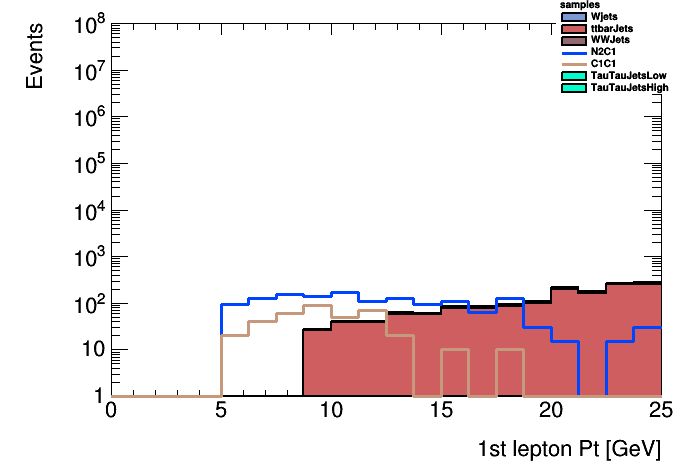
\includegraphics[width=0.3\textwidth]{h_PtMuons1st_2lead.png}
  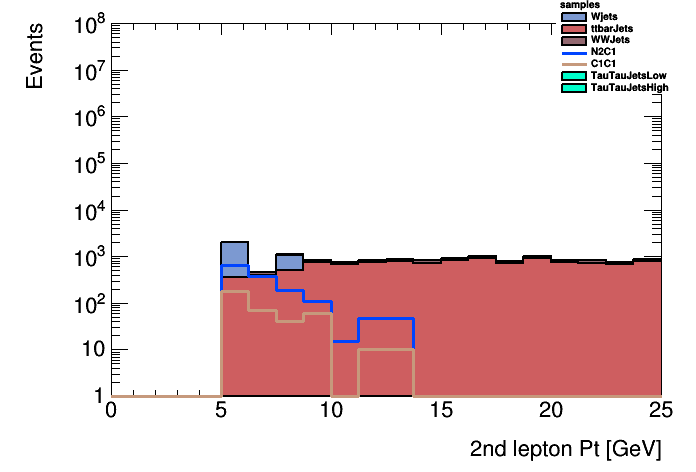
\includegraphics[width=0.3\textwidth]{h_PtMuons2nd_2lead.png}
  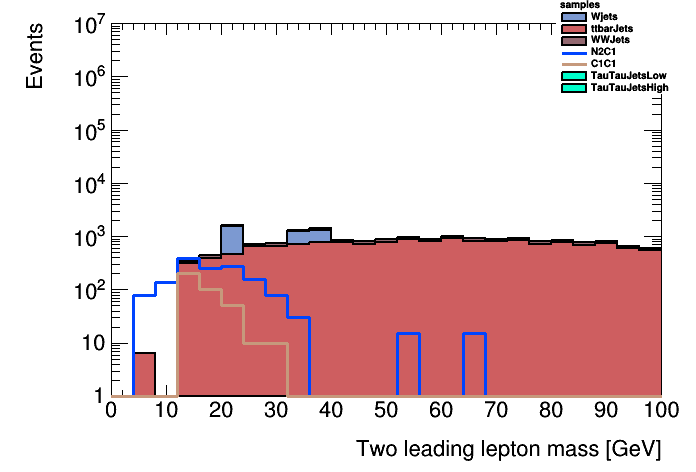
\includegraphics[width=0.3\textwidth]{h_llmass_2lead.png}
  \caption{The signal after selection. Leading lepton $p_{\rm T}$ (left), second leading lepton $p_{\rm T}$ (middle), first two leading lepton mass. SUSY signals (blue and orange lines), background processes (filled green, red, blue).}
  \label{fig:select}
\end{figure}

After this selection we see that indeed signal ratio is improved, but still a lot of background $pp \to t \bar t + j$ still is left which needs more carefull analysis on how it can be excluded. For significance calculation we use leading lepton transverse momentum in a region $5<p_{\rm T}<20~\rm{GeV}$ where results can be seen in \cref{tab:select}.
\begin{table}[!ht]
  \setlength{\tabcolsep}{12pt}
  \centering
  \begin{tabular}{l|rrrrrr}
    & $\tau \tau$ & $t \bar t$ & $WW$ & $W$ & $\chi_1^{\pm} \chi_1^{\pm}$ &  $\chi_1^{\pm} \chi_2^0$ \\
    \hline
    $Events_{L=3000~\rm{fb}^{-1}}$  & 0 & $758 \pm 27$ & $67 \pm 8$ & 0 & $370 \pm 19$ & $1422 \pm 38$ \\
    $\sigma_{L=300~\rm{fb}^{-1}}$ & - & - & - & - & 0 & 0 \\
    $\sigma_{L=3000~\rm{fb}^{-1}}$ & - & - & - & - & 0 & 0 
  \end{tabular}
  \caption{Significance calculation for luminosity $L=300~\rm{fb}^{-1}$ and $L=3000~\rm{fb}^{-1}$ with background uncertainty $30~\%$.
    %Number of events at $L=3000fb^-1$ after selection for leading lepton transverse momenta in region  for $L=3000fb$ and corresponding significance for luminosity $L=300 fb^-1$ and $L=3000 fb^-1$ with background uncertainty $30 \%$.
  }
  \label{tab:select}
\end{table}

\section{Conclussions}

\begin{itemize}
\item Wit selection used in this report we are able to better distinguish signal from background processes.  
\item SM process $pp \to t \bar t + j$ is not excluded efficiently enough with a present selection. A further study of how it can be minimized is needed. 
\item The significance discovering higgsino particle with mass $100~\rm{GeV}$ at HL LHC is ... which is (not) enough for making discovery. 
\end{itemize}

% \nocite{*}
%\bibliographystyle{unsrt}
\bibliography{bibliography}{9}
%\bibliographystyle{plain}
  \end{document}

%%% Local Variables:
%%% mode: latex
%%% TeX-master: t
%%% End:














